% !TEX root = ../../../main.tex
% 来源：中学数学实验教材·第三册（高中数学）
% 章节：三角函数的图象和性质 / 正弦函数的图象和性质
% 原始文件：7.tex，行 407-417
% 类型：tikz
% ---
    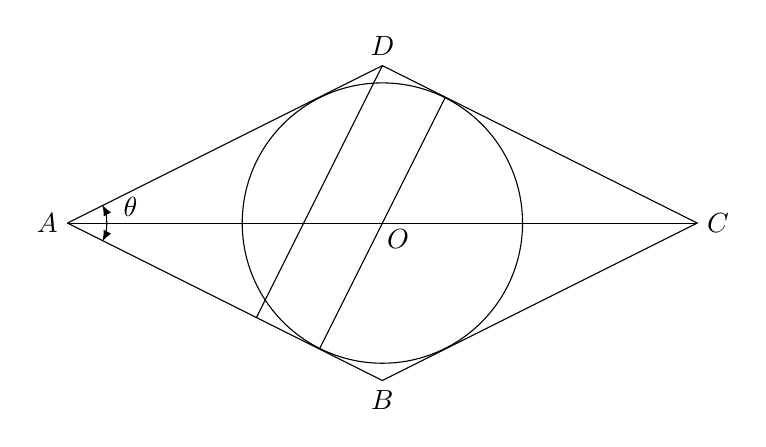
\begin{tikzpicture}[>=latex]
 \draw (-4,0)node[left]{$A$}--(0,2)node[above]{$D$}--(4,0)node[right]{$C$}--(0,-2)node[below]{$B$}--(-4,0)    ;
\draw (-4,0)--(4,0);
\draw (0,0) circle (1.78);       
\draw (.8,1.6)--(-.8,-1.6);
\draw (0,2)--(-1.6,-1.2);
\node at (.2,-.2){$O$};
\draw[->](-3.5,0) arc (0:28:.5);
\draw[->](-3.5,0) arc (0:-28:.5);
\node at (-3.2,0.2){$\theta$};
    \end{tikzpicture}
